%Hallo Andrin
% main.tex -- Paper zum Thema <parallelisierung>
%
% (c) 2020 Autor, OST Ostschweizer Fachhochschule
%
% !TEX root = ../../buch.tex
% !TEX encoding = UTF-8
%
\chapter{Thema\label{chapter:parallelisierung}}
\kopflinks{Thema}
\begin{refsection}
\chapterauthor{Andrin Kälin, Andrin Rütsche}

Ein paar Hinweise für die korrekte Formatierung des Textes
\begin{itemize}
\item
Absätze werden gebildet, indem man eine Leerzeile einfügt.
Die Verwendung von \verb+\\+ ist nur in Tabellen und Arrays gestattet.
\item
Die explizite Platzierung von Bildern ist nicht erlaubt, entsprechende
Optionen werden gelöscht. 
Verwenden Sie Labels und Verweise, um auf Bilder hinzuweisen.
\item
Beginnen Sie jeden Satz auf einer neuen Zeile. 
Damit ermöglichen Sie dem Versionsverwaltungssysteme, Änderungen
in verschiedenen Sätzen von verschiedenen Autoren ohne Konflikt 
anzuwenden.
\item 
Bilden Sie auch für Formeln kurze Zeilen, einerseits der besseren
Übersicht wegen, aber auch um GIT die Arbeit zu erleichtern.
\end{itemize}

\input{papers/parallelisierung/Lokalität.tex}
%
% teil1.tex -- Beispiel-File für das Paper
%
% (c) 2020 Prof Dr Andreas Müller, Hochschule Rapperswil
%
% !TEX root = ../../buch.tex
% !TEX encoding = UTF-8
%
\section{Metrik und Hodge-Theorie 
\label{maxwell:section:teil1}}
\kopfrechts{Metrik und Hodge-Theorie}

\subsection{Minkowski Metrik}
In der speziellen Relativitätstheorie (SRT) wird die Minkowski-Metrik verwendet.
\index{spezielle Relativitätstheorie}%
\index{Relativitätstheorie, spezielle}%
\index{Minkowski-Metrik}%
Da es in der SRT keine Krümmung und Gravitation gibt, sind alle Elemente ausserhalb der Diagonale des metrischen Tensors null und somit ist die Raum-Zeit flach.
Zwei Signaturen sind üblich.
Einerseits gibt es die $({-}{+}{+}{+})$-Signatur, bei welcher die Zeitkomponente negativ und die Raumkomponenten positiv gezählt werden.
Andererseits gibt es die $({+}{-}{-}{-})$-Signatur, bei welcher die Zeitkomponente positiv und die Raumkomponenten negativ gezählt werden.
Beide Signaturen sind gleichwertig, solange man sich auf eine Metrik festlegt und diese konsequent beibehält.
Im Folgenden werden wir uns an die $({-}{+}{+}{+})$-Signatur halten.
Daher definieren wir den metrischen Tensor als
\begin{equation}
	g^{ik} = \begin{pmatrix}
		-1 & 0 & 0 & 0 \\ 0 & 1 & 0 & 0 \\ 0 & 0 & 1 & 0 \\ 0 & 0 & 0 & 1 
	\end{pmatrix}.
	\label{maxwell:section:teil1:metrik}
\end{equation}
Der Ausdruck für ein Linienelement in dieser Metrik ist definiert als
\begin{equation*}
	dl^2 = -(dx^0)^2 +(dx^1)^2+(dx^2)^2+(dx^3)^2.
\end{equation*}
Damit wir Raum und Zeit in dieser Metrik gleichartig behandeln können, wählen wir beim Übergang in physikalische Einheiten 
\begin{equation}
	\label{maxwell:koordinaten}
	x^0 = ct,\quad x^1 = x,\quad x^2 = y, \quad x^3 = z .
\end{equation}
Dabei entspricht $c$ der Lichtgeschwindigkeit und ein Linienelement ist somit definiert als
\begin{equation*}
	dl^2 = -c^2dt^2 +dx^2+dy^2+dz^2.
\end{equation*}
Eine Konsequenz dieser Signatur ist, dass zeitartige Abstände $dl^2 < 0$ und raumartige Abstände $dl^2 > 0$ sind.

\subsection{Hodge-Duale der Basis-$k$-Formen}
Für den Teil der inhomogenen Maxwell-Gleichungen benötigen wir die Hodge-Duale von 1-Formen, 2-Formen und 3-Formen im vierdimensionalen Minkowski-Raum.
Um dabei die korrekten Vorzeichen zu erhalten, muss die Hodge-Dualität mit Hilfe des metrischen Tensors $g^{ik}$  der Minkowski-Metrik verwendet werden.

Wir verwenden die Definition des Hodge-Operators
\begin{equation*}
	\alpha \wedge \ast \beta = \langle \alpha, \beta \rangle \operatorname{vol}(M),
\end{equation*}
wobei $\langle \cdot , \cdot \rangle$ das durch die Metrik $g^{ik}$ induzierte Skalarprodukt ist.
Im Folgenden führen wir alle Berechnungen der Hodge-Duale von 1-, 2- und 3-Formen durch.
Wir verwenden $g^{ik}$ gemäss \eqref{maxwell:section:teil1:metrik} und $\operatorname{vol}(M) = dx^0 \wedge dx^1 \wedge dx^2 \wedge dx^3$.
\begin{definition}
\label{maxwell:hodge:kurzschreibweise}
Um die Notation kompakter und übersichtlicher zu gestalten, führen wir die Schreibweise
\begin{align*}
	dx^{i\!j} &:= dx^i \wedge dx^j, 
	%\label{maxwell:hodge:zwei}
	\\
	dx^{i\!jk} &:= dx^i \wedge dx^j \wedge dx^k, 
	%\label{maxwell:hodge:drei}
	\\
	dx^{i\!jkl} & := dx^i \wedge dx^j \wedge dx^k \wedge dx^l
	\notag
\end{align*}
für Wedge-Produkte von Basisformen ein.
\end{definition}
Mit dieser Vorbereitung können wir nun die konkreten Hodge-Duale der Basisformen berechnen.
\subsubsection{Hodge-Duale von 1-Formen}
\begin{align*}
	\ast dx^0 
	&= s \, dx^{123} \\
	dx^0 \wedge \ast dx^0 
	&= dx^0 \wedge s \, dx^{123} = s \, dx^{0123} \\
	&= \langle dx^0, dx^0 \rangle \operatorname{vol}(M) = g^{00} \, dx^{0123} = -dx^{0123} \\
	\Rightarrow s &= -1 \Rightarrow \boxed{\ast dx^0 = - dx^{123}}
	\\[1em]
	\ast dx^1 
	&= s \, dx^{023} \\
	dx^1 \wedge \ast dx^1 
	&= dx^1 \wedge s \, dx^{023} = -s \, dx^{0123} \\
	&= \langle dx^1, dx^1 \rangle \operatorname{vol}(M) = g^{11} \, dx^{0123} = dx^{0123} \\
	\Rightarrow s &= -1 \Rightarrow \boxed{\ast dx^1 = - dx^{023}}
	\\[1em]
	\ast dx^2 
	&= s \, dx^{013} \\
	dx^2 \wedge \ast dx^2 
	&= dx^2 \wedge s \, dx^{013} = s \, dx^{0123} \\
	&= \langle dx^2, dx^2 \rangle \operatorname{vol}(M) = g^{22} \, dx^{0123} = dx^{0123} \\
	\Rightarrow s &= +1 \Rightarrow \boxed{\ast dx^2 = dx^{013}}
	\\[1em]
	\ast dx^3 
	&= s \, dx^{012} \\
	dx^3 \wedge \ast dx^3 
	&= dx^3 \wedge s \, dx^{012} = -s \, dx^{0123} \\
	&= \langle dx^3, dx^3 \rangle \operatorname{vol}(M) = g^{33} \, dx^{0123} = dx^{0123} \\
	\Rightarrow s &= -1 \Rightarrow \boxed{\ast dx^3 = - dx^{012}}
\end{align*}

\subsubsection{Hodge-Duale von 2-Formen}
\begin{align*}
	\ast dx^{01} &= s \, dx^{23} \\
	dx^{01} \wedge \ast dx^{01} &= s \, dx^{0123} \\
	&= \langle dx^{01}, dx^{01} \rangle \, \operatorname{vol}(M) 
	= g^{00} g^{11} \operatorname{vol}(M) = -dx^{0123} \\
	\Rightarrow s &= -1 \Rightarrow \boxed{\ast dx^{01} = - dx^{23}}
	\\[1em]
	\ast dx^{12} &= s \, dx^{03} \\
	dx^{12} \wedge \ast dx^{12} &= s \, dx^{0123} \\
	&= \langle dx^{12}, dx^{12} \rangle \, \operatorname{vol}(M) 
	= g^{11} g^{22} \operatorname{vol}(M) = dx^{0123} \\
	\Rightarrow s &= +1 \Rightarrow \boxed{\ast dx^{12} = dx^{03}}
	\\[1em]
	\ast dx^{23} &= s \, dx^{01} \\
	dx^{23} \wedge \ast dx^{23} &= s \, dx^{0123} \\
	&= \langle dx^{23}, dx^{23} \rangle \, \operatorname{vol}(M) 
	= g^{22} g^{33} \operatorname{vol}(M) = dx^{0123} \\
	\Rightarrow s &= +1 \Rightarrow \boxed{\ast dx^{23} = dx^{01}}
	\\[1em]
	\ast dx^{02} &= s \, dx^{13} \\
	dx^{02} \wedge \ast dx^{02} &= -s \, dx^{0123} \\
	&= \langle dx^{02}, dx^{02} \rangle \, \operatorname{vol}(M) 
	= g^{00} g^{22} \operatorname{vol}(M) = -dx^{0123} \\
	\Rightarrow s &= +1 \Rightarrow \boxed{\ast dx^{02} = dx^{13}}
	\\[1em]
	\ast dx^{03} &= s \, dx^{12} \\
	dx^{03} \wedge \ast dx^{03} &= s \, dx^{0123} \\
	&= \langle dx^{03}, dx^{03} \rangle \, \operatorname{vol}(M) 
	= g^{00} g^{33} \operatorname{vol}(M) = -dx^{0123} \\
	\Rightarrow s &= -1 \Rightarrow \boxed{\ast dx^{03} = - dx^{12}}
	\\[1em]
	\ast dx^{13} &= s \, dx^{02} \\
	dx^{13} \wedge \ast dx^{13} &= -s \, dx^{0123} \\
	&= \langle dx^{13}, dx^{13} \rangle \, \operatorname{vol}(M) 
	= g^{11} g^{33} \operatorname{vol}(M) = dx^{0123} \\
	\Rightarrow s &= -1 \Rightarrow \boxed{\ast dx^{13} = - dx^{02}}
\end{align*}

\subsubsection{Hodge-Duale von 3-Formen}
\begin{align*}
	\ast dx^{012} &= s \, dx^3 \\
	dx^{012} \wedge \ast dx^{012} &= s \, dx^{0123} \\
	&= \langle dx^{012}, dx^{012} \rangle \, \operatorname{vol}(M) 
	= g^{00} g^{11} g^{22} \operatorname{vol}(M) = -dx^{0123} \\
	\Rightarrow s &= -1 \Rightarrow \boxed{\ast dx^{012} = - dx^3}
	\\[1em]
	\ast dx^{013} &= s \, dx^2 \\
	dx^{013} \wedge \ast dx^{013} &= -s \, dx^{0123} \\
	&= \langle dx^{013}, dx^{013} \rangle \, \operatorname{vol}(M) 
	= g^{00} g^{11} g^{33} \operatorname{vol}(M) = -dx^{0123} \\
	\Rightarrow s &= 1 \Rightarrow \boxed{\ast dx^{013} = dx^2}
	\\[1em]
	\ast dx^{023} &= s \, dx^1 \\
	dx^{023} \wedge \ast dx^{023} &= s \, dx^{0123} \\
	&= \langle dx^{023}, dx^{023} \rangle \, \operatorname{vol}(M) 
	= g^{00} g^{22} g^{33} \operatorname{vol}(M) = -dx^{0123} \\
	\Rightarrow s &= -1 \Rightarrow \boxed{\ast dx^{023} = - dx^1}
	\\[1em]
	\ast dx^{123} &= s \, dx^0 \\
	dx^{123} \wedge \ast dx^{123} &= -s \, dx^{0123} \\
	&= \langle dx^{123}, dx^{123} \rangle \, \operatorname{vol}(M)
	= g^{11} g^{22} g^{33} \operatorname{vol}(M) = dx^{0123} \\
	\Rightarrow s &= -1 \Rightarrow \boxed{\ast dx^{123} = - dx^0}
\end{align*}
In der Tabelle \ref{maxwell:section:teil1:Hodge-Tabelle} sind alle berechneten Hodge-Duale noch einmal zusammengefasst.
\begin{table}
	\centering
	%\caption{Hodge-Duale}
	%\label{maxwell:section:teil1:Hodge-Tabelle}
	\begin{tabularx}{\textwidth}{ 
			| >{\centering\arraybackslash}X 
			| >{\centering\arraybackslash}X 
			| >{\centering\arraybackslash}X | }
		\hline
		\textbf{1-Form} & \textbf{2-Form} & \textbf{3-Form} \\
		\hline
		\( \rule{0pt}{1.5em} {\ast} dx^0 = -dx^1 \wedge dx^2 \wedge dx^3 \) \newline
	\( {\ast} dx^1 = -dx^0 \wedge dx^2 \wedge dx^3 \) \newline
	\( {\ast} dx^2 = \phantom{-} dx^0 \wedge dx^1 \wedge dx^3 \) \newline
	\( {\ast} dx^3 = -dx^0 \wedge dx^1 \wedge dx^2 \, \) 
	&
	\( \rule{0pt}{1.5em} {\ast} (dx^0 \wedge dx^1) = -dx^2 \wedge dx^3 \) \newline
	\( {\ast} (dx^1 \wedge dx^2) = \phantom{-} dx^0 \wedge dx^3 \) \newline
	\( {\ast} (dx^2 \wedge dx^3) = \phantom{-} dx^0 \wedge dx^1 \) \newline
	\( {\ast} (dx^0 \wedge dx^2) = \phantom{-} dx^1 \wedge dx^3 \) \newline
	\( {\ast} (dx^0 \wedge dx^3) = -dx^1 \wedge dx^2 \) \newline
	\( {\ast} (dx^1 \wedge dx^3) = -dx^0 \wedge dx^2 \)
	&
	\( \rule{0pt}{1.5em} {\ast} (dx^0 \wedge dx^1 \wedge dx^2) = -dx^3 \) \newline
	\( {\ast} (dx^0 \wedge dx^1 \wedge dx^3) = \phantom{-} dx^2 \) \newline
	\( {\ast} (dx^0 \wedge dx^2 \wedge dx^3) = -dx^1 \) \newline
	\( {\ast} (dx^1 \wedge dx^2 \wedge dx^3) = -dx^0 \)
		\\
		\hline
	\end{tabularx}
	\caption{Tabelle aller Hodge-Duale von 1-, 2-, und 3-Formen mit $({-}{+}{+}{+})$-Signatur}
	\label{maxwell:section:teil1:Hodge-Tabelle}
\end{table}








%Hast du gut gemacht
% einleitung.tex -- Beispiel-File für die Einleitung
%
% (c) 2020 Prof Dr Andreas Müller, Hochschule Rapperswil
%
% !TEX root = ../../buch.tex
% !TEX encoding = UTF-8
\section{Gebietsunterteilung}
\label{parallelisierung:sec:Gebietsunterteilung}
\kopfrechts{Gebietsunterteilung}


\subsection{Motivation}
Wie aus dem Abschnitt der numerischen Methoden hervorgeht, führt eine Verfeinerung der Raum- und Zeitauflösung zwar zu genaueren Ergebnissen, jedoch auch zu mehr Datenpunkten und somit einem erheblich höheren Rechenaufwand. 
Mit zunehmender Gitterfeinheit steigt die Anzahl der Unbekannten quadratisch (in 2D) bzw. kubisch (in 3D).  
Um diese steigende Komplexität effizient bewältigen zu können, bietet sich die Gebietsunterteilung an.

Feldgleichungen wie die Wärmeleitungsgleichung besitzen wie im ersten Abschnitt dieser Arbeit erklärt eine lokale Struktur.
Also hängt der Wert in einem Gitterpunkt nur von seinen direkten Nachbarn (räumlich und zeitlich) ab.  
Diese Eigenschaft erlaubt es, ein grosses Problem in kleinere Teilprobleme zu zerlegen, sie getrennt zu berechnen und anschliessend wieder zusammenzufügen.

\subsection{Mathematische Zerlegung}
Sei $\Omega \subset {R}^2$ das Gesamtgebiet, diskretisiert durch ein kartesisches Gitter.  
Nun zerlegen wir $\Omega$ in $P$ disjunkte Teilgebiete $\Omega_p$:
\begin{equation}
	\Omega = \bigcup_{p=1}^P \Omega_p,
	\qquad 
	\Omega_p \cap \Omega_q = \emptyset \quad \text{für } p \neq q.
\end{equation}

Das bedeutet:
\begin{itemize}
	\item Das Gesamtgebiet setzt sich vollständig aus den Teilgebieten zusammen.
	\item Jedes Gitterelement gehört genau zu einem Teilgebiet.
	\item Die Teilgebiete überlappen sich nicht, können sich aber an den Rändern berühren.
\end{itemize}

Anschaulich entspricht dies einem Puzzle: 
jedes Teilgebiet ist ein Puzzlestück, das nahtlos mit den Nachbarstücken zusammenpassen muss.

\subsection{Kopplungsbedingungen}
Damit die Zerlegung konsistent bleibt, müssen an den Schnittstellen (Rändern) bestimmte Bedingungen erfüllt sein:

\paragraph{Stetigkeit der Lösung.}
\index{Stetigkeit der Lösung}%
\begin{equation}
	T_{\Omega_p}(x,y,t) = T_{\Omega_q}(x,y,t)
	\qquad \forall (x,y) \in \partial \Omega_p \cap \partial \Omega_q.
\end{equation}
Die Temperatur darf an den Schnittkanten keine Sprünge zeigen.

\paragraph{Stetigkeit des Flusses.}
\index{Stetigkeit des Flusses}%
\begin{equation}
	- \kappa \, \nabla T_{\Omega_p} \cdot n
	=
	- \kappa \, \nabla T_{\Omega_q} \cdot n
	\qquad \forall (x,y) \in \partial \Omega_p \cap \partial \Omega_q.
\end{equation}
Es darf keine künstliche Wärmequelle oder -senke entstehen: der aus einem Gebiet austretende Fluss tritt ins Nachbargebiet ein.

\subsection{Diskrete Umsetzung mit Ghost-Zellen}
Betrachten wir erneut die zweidimensionale Wärmeleitungsgleichung
\begin{equation}
	\frac{\partial T}{\partial t} = 
	\alpha \left(
	\frac{\partial^2 T}{\partial x^2} + \frac{\partial^2 T}{\partial y^2}
	\right).
\end{equation}
Zur Wiederholung: Mit FDM ergibt sich für ein quadratisches Gitter mit $\Delta l=\Delta x=\Delta y$ die Update-Formel
\begin{equation}
	T_{i,j}^{n+1}
	=
	T_{i,j}^{n}
	+
	\lambda \left(
	T_{i+1,j}^{n}+T_{i-1,j}^{n}+T_{i,j+1}^{n}+T_{i,j-1}^{n}-4\,T_{i,j}^{n}
	\right),
	\quad
	\lambda=\frac{\alpha\Delta t}{(\Delta l)^2}.
	\label{eq:update-dd}
\end{equation}

Für innere Punkte eines Teilgebiets $\Omega_p$ kann \eqref{eq:update-dd} direkt berechnet werden.  
An Schnittkanten hingegen benötigt man Werte aus Nachbargebieten.  
Dazu führt man sogenannte Ghost-Zellen ein:
\begin{itemize}
	\item Sie enthalten Kopien der Randwerte aus benachbarten Teilgebieten.
	\item Nach jedem Zeitschritt werden sie synchronisiert.
\end{itemize}
So kann jedes Teilgebiet lokal weiterrechnen. Dies erlaubt eine effiziente Parallelisierung, da nur die Schnittkanten kommuniziert werden müssen.

Abbildung~\ref{parallelisierung:fig:ghostCells} zeigt exemplarisch, wie an den Rändern benachbarter Teilgebiete Daten ausgetauscht werden. Farblich orange hervorgehoben sind die Ghost-Zellen.

\begin{figure}
	\centering
	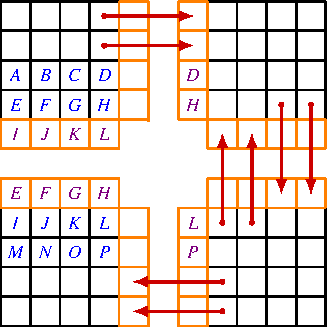
\includegraphics{papers/parallelisierung/images/ghostCells.pdf}
	\caption{Funktionsweise der Ghost-Zellen}
	\label{parallelisierung:fig:ghostCells}
\end{figure}



\subsection{Speziallfall: Stationärer Grenzfall}
Für $n \to \infty$ strebt das Zeitschrittverfahren gegen ein stationäres Temperaturfeld. 
Dann verschwindet die Zeitableitung, und die Wärmeleitungsgleichung reduziert sich auf die Laplace-Gleichung
\[
\nabla^2 T = 0.
\]

Diskretisiert mit FDM erhält man für jeden inneren Gitterpunkt eine lineare Beziehung zu seinen Nachbarn:
\[
-4T_{i,j} + T_{i+1,j} + T_{i-1,j} + T_{i,j+1} + T_{i,j-1} = 0.
\]

Alle diese Gleichungen zusammen bilden ein lineares System
\[
\mathbf{A}\vec{u} = \vec{b}.
\]

\subsubsection{Beispiel: $5\times 5$-Gitter}

Einmal mehr legen wir uns ein Beispiel zurecht um dies besser zu verstehen. Dieses mal nehmen wir  ein $5\times 5$-Gitter mit folgenden Randwerten:
\[
T=100^\circ\mathrm{C}\ \text{(links)},\quad
T=0^\circ\mathrm{C}\ \text{(rechts)},\quad
T=80^\circ\mathrm{C}\ \text{(oben)},\quad
T=20^\circ\mathrm{C}\ \text{(unten)}.
\]
\begin{figure}
	\centering
	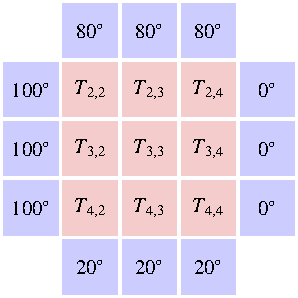
\includegraphics{papers/parallelisierung/images/stationaer.pdf}
	\caption{Beispiel-Setup $5\times5$-Grid für den stationären Grenzfall}
	\label{parallelisierung:fig:stationaer}
\end{figure}
Daraus ergeben sich $3\times 3 = 9$ innere Unbekannte.
Zusätzlich entfernen wir aus Gründen der Übersicht die Randzellen ohne Einfluss auf die inneren Zellen. Somit resultiert das Modell gemäss Abbildung \ref{parallelisierung:fig:stationaer}.


\subsubsection*{Diskretisierung}
Wenden wir nun die zuvor hergeleitete explizite Updateformel \eqref{eq:update-dd} auf dieses Gitter an, resultieren die folgenden 9 Gleichungen:
\begin{equation*}
\renewcommand{\arraycolsep}{3pt}
\begin{array}{cclclclclcl}
	-4\color{darkred}{T_{2,2}} &+& T_{3,2} &+& 80      &+& T_{2,3} &+& 100     &=& 0, \\
	-4\color{darkred}{T_{2,3}} &+& T_{3,3} &+& 80      &+& T_{2,4} &+& T_{2,2} &=& 0, \\
	-4\color{darkred}{T_{2,4}} &+& T_{3,4} &+& 80      &+& 0       &+& T_{2,3} &=& 0, \\
	-4\color{darkred}{T_{3,2}} &+& T_{4,2} &+& T_{2,2} &+& T_{3,3} &+& 100     &=& 0, \\
	-4\color{darkred}{T_{3,3}} &+& T_{4,3} &+& T_{2,3} &+& T_{3,4} &+& T_{3,2} &=& 0, \\
	-4\color{darkred}{T_{3,4}} &+& T_{4,4} &+& T_{2,4} &+& 0       &+& T_{3,3} &=& 0, \\
	-4\color{darkred}{T_{4,2}} &+& 20      &+& T_{3,2} &+& T_{4,3} &+& 100     &=& 0, \\
	-4\color{darkred}{T_{4,3}} &+& 20      &+& T_{3,3} &+& T_{4,4} &+& T_{4,2} &=& 0, \\
	-4\color{darkred}{T_{4,4}} &+& 20      &+& T_{3,4} &+& 0       &+& T_{4,3} &=& 0.
\end{array}
\end{equation*}

\subsubsection*{Matrixformulierung}
Wir ordnen die Unbekannten zeilenweise:
\[
\vec{u} =
\begin{pmatrix}
	T_{2,2}\\T_{2,3}\\T_{2,4}\\
	T_{3,2}\\T_{3,3}\\T_{3,4}\\
	T_{4,2}\\T_{4,3}\\T_{4,4}
\end{pmatrix}.
\]
Dann gilt:
\[
\mathbf{A}\vec{u}=\vec{b},
\]
mit
\[
\mathbf{A}=
\begin{pmatrix*}[r]
	-4& 1& 0& 1& 0& 0& 0& 0& 0\\
	1&-4& 1& 0& 1& 0& 0& 0& 0\\
	0& 1&-4& 0& 0& 1& 0& 0& 0\\
	1& 0& 0&-4& 1& 0& 1& 0& 0\\
	0& 1& 0& 1&-4& 1& 0& 1& 0\\
	0& 0& 1& 0& 1&-4& 0& 0& 1\\
	0& 0& 0& 1& 0& 0&-4& 1& 0\\
	0& 0& 0& 0& 1& 0& 1&-4& 1\\
	0& 0& 0& 0& 0& 1& 0& 1&-4
\end{pmatrix*},
\quad
\vec{b}=
\begin{pmatrix*}[r]
	-180\\-80\\-80\\
	-100\\0\\0\\
	-120\\-20\\-20
\end{pmatrix*}.
\]

\subsubsection*{Interpretation und Lösung}
\begin{itemize}
	\item $\mathbf{A}$ ist dünnbesetzt und spiegelt die 5-Punkt-Nachbarschaft wider.
	\item $\vec{b}$ enthält die Beiträge der Randwerte (verschieden je nach Position).
	\item Das System besitzt eine eindeutige Lösung: es liefert eine schräg verlaufende Temperaturverteilung zwischen den warmen und kalten Rändern.
\end{itemize}

\subsubsection*{Bemerkung zur Gebietsunterteilung im stationären Fall.}  
Im zeitabhängigen Fall werden Ghost-Zellen bei jedem Zeitschritt mit den Werten der Nachbargebiete gefüllt.  
Im stationären Fall dagegen gibt es keine Iteration in der Zeit, sodass die Ghost-Werte nicht direkt verfügbar sind.  
Um die Kopplung zwischen Subdomains herzustellen, gibt es zwei grundsätzliche Ansätze:

\begin{itemize}
	\item \emph{Algebraischer Ansatz:}  
	Das Gesamtsystem wird als grosse Blockmatrix aufgestellt.  
\index{Blockmatrix}%
	Jeder Hauptdiagonalblock \(A_{pp}\) beschreibt die inneren Zusammenhänge (die ``Selbstkopplung'') innerhalb eines Teilgebiets~\(\Omega_p\).  
\index{Hauptdiagonalblock}%
\index{Nebendiagonalblock}%
	Die Nebendiagonalblöcke \(C_{pq}\) modellieren die Kopplungen zu den Nachbargebieten~\(\Omega_q\).  
	
	Zur Illustration nehmen wir ein Beispiel mit drei Teilgebieten.  
	Das Gesamtsystem hat dann die Form
	\[
	\mathbf{A} =
	\begin{bmatrix}
		A_{11} & C_{12} & C_{13} \\
		C_{21} & A_{22} & C_{23} \\
		C_{31} & C_{32} & A_{33}
	\end{bmatrix}
	\]
	Hier enthält jeder Block \(A_{pp}\) die Koeffizienten für die inneren Punkte von~\(\Omega_p\), 
	während \(C_{pq}\) nur Einträge für die Schnittkanten trägt.  
	
	Durch Verfahren wie das Schur-Komplement kann die Lösung des Gesamtsystems auf die Werte an den Interfaces reduziert werden, 
\index{Schur-Komplement}%
	wodurch die Rechenlast deutlich sinkt.  
	Weiterführende Details finden sich beispielsweise in \cite{parallelisierung:smith1996}.
	
	\item \emph{Iterative Ansätze:}  
	Domain-Decomposition-Verfahren berechnen die Teilgebiete wiederholt und tauschen dabei nach jeder Iteration die Werte an den Schnittkanten aus, bis Konsistenz erreicht ist.  
	
	Ein klassisches Beispiel ist die \emph{Schwarz-Methode}.  
\index{Schwarz-Methode}%
	Hier werden an den künstlichen Rändern zwischen den Teilgebieten \emph{Dirichlet-Randbedingungen} vorgegeben, d.\,h.\ die benachbarten Teilgebiete liefern feste Temperaturwerte, die als Randwerte eingesetzt werden.  
\index{Dirichlet-Randbedingungen}%
	Genau diese Art von Randbedingungen haben wir auch im obigen Beispiel mit festen Temperaturen an den Aussenrändern des Gitters verwendet.  
	Die Schwarz-Methode ist einfach und robust, kann jedoch bei vielen Teilgebieten langsam konvergieren.  
	Eine ausführliche Darstellung findet sich in \cite{parallelisierung:quarteroniValli1999}.  
	
	Eine leistungsfähigere Alternative ist die \emph{Neumann--Neumann-Methode}.  
	In diesem Verfahren werden an den Schnittkanten \emph{Neumann-Randbedingungen} eingesetzt, also Bedingungen für die Flüsse (z.\,B.\ Wärmeströme) über die Gebietsgrenzen hinweg.  
\index{Neumann-Randbedingungen}%
	Die Subdomänen werden parallel berechnet, und die Flusswerte an den Interfaces werden iterativ korrigiert, bis Konsistenz erreicht ist.  
	Dieser Ansatz eignet sich besonders für elliptische Probleme und skaliert gut auf parallelen Rechnerarchitekturen.  
	Details hierzu finden sich in \cite{parallelisierung:gander2019}.
\end{itemize}


\subsection{Praktische Aspekte}

\subsubsection {Lastverteilung und Kommunikation}
Die Kosten pro Zeitschritt sind proportional zur Anzahl der Gitterpunkte im Teilgebiet 
($\mathcal{O}(|\Omega_p|)$).  
Die Kommunikationskosten entstehen durch den Austausch von Ghost-Zellen und hängen von der Länge der Schnittkante ab.  
\index{Kommunikationskosten}%
Für eine effiziente Parallelisierung ist es daher vorteilhaft, Teilgebiete mit möglichst kleinem 
Umfang/Flächen-Verhältnis zu wählen.  
In 2D bedeutet dies, dass quadratische Teilgebiete günstiger sind als lange, schmale Streifen.
Im 3D-Fall spricht man analog vom Oberflächen/Volumen-Verhältnis.  

\subsubsection {Stabilität}
Die Stabilitätskriterien der expliziten Finite-Differenzen-Methode gelten auch bei der Gebietsunterteilung unverändert.  
Insbesondere muss in 2D für ein quadratisches Gitter stets
\[
\lambda = \frac{\alpha \Delta t}{(\Delta l)^2} \leq \tfrac{1}{4}
\]
gelten.  
Diese Bedingung ist lokal in jedem Teilgebiet genauso einzuhalten wie global. 


%
% teil2.tex -- Beispiel-File für teil2 
%
% (c) 2020 Prof Dr Andreas Müller, Hochschule Rapperswil
%
% !TEX root = ../../buch.tex
% !TEX encoding = UTF-8
%
\section{Parallelisierung
\label{parallelisierung:sec:Parallelisierung}}
\kopfrechts{Parallelisierung}
Wir kennen nun numerische Verfahren, welche es einer Maschine erlaubt unsere Feldgleichungen zu berechnen.
Wir wissen auch, wie wir unser Feld in Teilgebiete unterteilen können.
Das gibt uns alle Werkzeuge, welche wir benötigen um die Berechnungen unserer Gleichungen auf mehrere Maschinen aufzuteilen.

Bei der Parallelisierung von Feldgleichungen in einem Multiprozessorsystem wird jedem Prozessor eines oder mehrere zusammenhängende Teilgebiete zugewiesen.
Die Teilgebiete müssen theoretisch nicht zusammenhängend sein aber um die Kommunikation zwischen Prozessoren zu minimieren ist dieses Vorgehen sinnvoll und üblich.
Da die Randzellen jedes Teilgebietes abhängig von den angrenzenden Zellen sind, siehe \ref{parallelisierung:sec:Gebietsunterteilung}, müssen die vorhandenen Informationen dieser Zellen zwischen Gebieten auf unterschiedlichen Prozessoren ausgetauscht werden.
Dieser Austausch ist mit erheblichem zeitlichen Aufwand verbunden.
Die Frage, wie fein ein Gitter in verschiedene Teilgebiete aufgeteilt werden soll, ist also immer eine optimierungs-Frage.
Man muss ein Optimum finden, wo der zeitliche Gewinn der parallelen Berechnung die zeitlichen Verluste der Interprozess-Kommunikation überwiegen.

%
% einleitung.tex -- Beispiel-File für die Einleitung
%
% (c) 2020 Prof Dr Andreas Müller, Hochschule Rapperswil
%
% !TEX root = ../../buch.tex
% !TEX encoding = UTF-8
%
\subsection{Kommunikation zwischen Gebieten
\label{parallelisierung:sub:Interprozess}}
Zuerst eine kurze Rekapitulation zu einigen Begrifflichkeiten, welche wichtig sind für die Welt der parallelen Programmierung.
Ein Prozessor ist eine physische Recheneinheit wie zum Beispiel eine CPU oder GPU.
Prozessoren sind meist aus mehreren Kernen aufgebaut.
Jeder Kern ist eine eigenständige Recheneinheit und hat privaten wie auch mit anderen Kernen geteilten Speicher.
Ein Prozess ist ein eigenständiges Programm, welches vom Betriebssystem alle nötigen Resourcen wie Speicher, Rechenzeit und Daten zugeteilt bekommt.
Threads sind Teilaufgaben eines Prozesses, die gleichzeitig auf den verschiedenen Kernen des Prozessors arbeiten und sich die Daten und den Speicher dieses Prozesses teilen.

Für das Austauschen von Daten zwischen Teilgebieten gibt es zwei häufig verwendete Parallele Programmier- und Kommunikationsschnittstellen, OpenMP und MPI.
Im folgen werden beide kurz vorgestellt.

\subsubsection{OpenMP}
OpenMP ist eine API, welche sehr einfach das erzeugen von Threads und die Kommunikation zwischen diesen ermöglicht.
Jedes Teilgebiet wird hier einem Thread zugeteilt. 
Da sich diese Threads den Speicher des Prozesses teilen, nutzt OpenMP Shared-Memory für den Austausch von Daten.
Bei OpenMP gibt es keinen Thread-eigenen Speicher.
Jeder Thread kann also auf die Randzellen anderer Threads zugreifen.
Dadurch benötigt es keine Kommunikation zwischen den Teilgebieten im engeren Sinn.

Für kleine Systeme ist OpenMP eine einfache und gute Lösung.
Da es aber auf Shared-Memory basiert ist es schlecht skalierbar.
Werden für grosse Berechnungen mehrere Prozessoren verwendet ist Shared-Memory oft nicht verfügbar.
Grosse Berechnungen möchte man oft auch auf verschiedene Maschinen aufteilen, was mit OpenMP nicht möglich ist.
Der einfache Aufbau für den Programmierer bedeutet außerdem weniger Kontrolle über die Datenverteilung.

\subsubsection{MPI}
MPI ist ein Message Passing Interface.
Es dient nicht dazu Prozesse oder threads zu erzeugen.
Diese Aufgabe muss vom Betriebssystem ausgeführt werden.

MPI stellt Funktionen zur Verfügung für eine effiziente Kommunikation mittels Nachrichten zwischen den Prozessen.
Diese Prozesse haben nicht zwingend einen Shared Memory bereich.
Es wird daher als Distributed-Memory-Programmiermodell bezeichnet.
Jedes Teilgebiet wird hier einem Prozess zugeteilt.
Die Informationen über angrenzende Teilgebiete wird mittels Nachrichten oder auch Messages zwischen den Prozessen ausgetauscht.
Der Programmierer muss explizit Datenverteilung und Kommunikation steuern, was zwar einiges mehr Programmieraufwand aber auch bessere Kontrolle über die Daten bedeutet.

MPI zeichnet sich besonders über eine gute Skalierbarkeit aus.
Da kein Shared Memory nötig ist, kann man über beliebig viele Knoten, zum Beispiel mehrere CPUs oder ganze Rechner, die Daten durch Messages austauschen.

Man kann MPI auch für Systeme mit Shared Memory als eine Art Universallösung verwenden.
In diesem Fall wird allerdings trotz einem geteiltem Speicherbereich erheblicher Overhead für Kommunikation produziert, welcher mit OpenMP vermieden werden könnte.
%
% einleitung.tex -- Beispiel-File für die Einleitung
%
% (c) 2020 Prof Dr Andreas Müller, Hochschule Rapperswil
%
% !TEX root = ../../buch.tex
% !TEX encoding = UTF-8
%
\subsection{Prozess Synchronisation \label{parallelisierung:subsection:Synchronisation}}
Lorem ipsum dolor sit amet, consetetur sadipscing elitr, sed diam
nonumy eirmod tempor invidunt ut labore et dolore magna aliquyam
erat, sed diam voluptua \cite{parallelisierung:bibtex}.
At vero eos et accusam et justo duo dolores et ea rebum.
Stet clita kasd gubergren, no sea takimata sanctus est Lorem ipsum
dolor sit amet.

Lorem ipsum dolor sit amet, consetetur sadipscing elitr, sed diam
nonumy eirmod tempor invidunt ut labore et dolore magna aliquyam
erat, sed diam voluptua.
At vero eos et accusam et justo duo dolores et ea rebum.  Stet clita
kasd gubergren, no sea takimata sanctus est Lorem ipsum dolor sit
amet.




\subsection{Beispiel an der allgemeinen Wärmeleitungsgleichung
\label{parallelisierung:sub:BeispielParallelisierung}}
Zum besseren Verständnis wollen wir mit OpenMP ein Konkretes Beispiel für die Parallelisierung der allgemeinen Wärmeleitungsgleichung realisieren.
Zum Vergleich wird auch die Serielle Vorgehensweise präsentiert.
Als Ausgangslage soll für ein Gitter von AxB Zellen C Updates durchgeführt werden.
Für jedes Update wird die Formel \ref{parallelisierung:eq:update_formel} aus Abschnitt \ref{parallelisierung:sec:update_formel} verwendet.
Links und Rechts der Zellen gibt es Reihen mit unveränderlicher Temperatur, welche einen Heiz- respektive Kühlkörper darstellen.
Ober- und unterhalb der Zellen gibt es Zeilen mit unveränderlicher Temperatur, welche die Umgebungstemperatur darstellen.
Diese Konstanten, wie auch $\lambda$ als Konstante für die Updateformel können alle im Main-File des Programms definiert werden und sind unveränderlich.

Beide Lösungen verwenden Arrays zur Zwischenspeicherung der Zellen.
Für Arrays werden gerne Vektoren aus der C++ Standar Library (STL) verwendet.
Für ein zweidimensionales Array wird zum Beispiel
\begin{lstlisting}
	std::vector<std::vector<double>> grid;
\end{lstlisting}
benützt.
Man muss sich allerdings bewusst sein, dass diese Variante keinen kontinuierlichen Bereich im Speicher reserviert.
Diese Variante speichert zuerst ein äußeres Array (Zeilen), und jede Zeile allokiert separat ihren eigenen Speicher.
Das verschlechtert enorm die Cache-Lokalität des Programms und damit die Performanz.
Als elegantere Lösung verwendet man bei numerischen Verfahren für partielle Differentialgleichungen eindimensionale Arrays und rechnet die Indizes mittels inline-Funktion um.
\begin{lstlisting}
	std::vector<double> grid(nx * ny);
	
	inline double& at(int i, int j) {
		return grid[i * nx + j];  // Row-major
	}
\end{lstlisting}
Damit garantiert man eine kontinuierliche Speicherung der Daten.

\subsubsection{Serielle Lösung}
\label{parallelisierung:sub:serLoesung}}
Zur Vorbereitung werden Zwei Arrays der Grösse 
\begin{equation}
	A+2 * B+2 
\end{equation}
angelegt. 

\begin{lstlisting}
	std::vector<double> grid(A * B);
	std::vector<double> gridNew(A * B);
\end{lstlisting}
Die Addition von zwei ist notwendig, um die Umgebenden Temperaturen speichern zu können.
In beiden Arrays wird nun die Umgebungstemperatur in die erste und letzte Zeile geschrieben.
Die jeweilige Temperatur der Heiz-/Kühlkörper wird in die erste und letzte Spalte geschrieben.
Das erste Array wird für die aktuellen Temperaturen der Zellen verwendet.
Als Ausgangspunkt kann in dieses die Umgebungstemperatur eingetragen werden.
Mit einer Schlaufe kann nun für alle A*B Zellen der neue Wert mit der Updateformel berechnet und in die entsprechende Zelle im zweiten Array geschrieben werden.
\begin{lstlisting}[caption={Update-Schritt (seriell)},label={parallelisierung:code:updateSeriel}]
	for (int i = 1; i < B - 1; ++i) {     // ueberspringt erste und letzte Zeile
		const int row = i * A;
		for (int j = 1; j < A - 1; ++j) { // ueberspringt erste und letzte Spalte
			const int idx   = row + j;
			const int up    = idx - A;
			const int down  = idx + A;
			const int left  = idx - 1;
			const int right = idx + 1;
			
			nextTemp[idx] = currentTemp[idx]
			+ lambda * (src[up] + src[down] + src[left] + src[right]
			- 4.0 * src[idx]);
		}
	}
\end{lstlisting}
Im Beispiel ist src ein Pointer auf das Array mit den aktuellen Werten und dst ist ein Pointer auf das Array mit den neuen Werten.
Bei der Verwendung von Vektoren erhält man die Adresse des ersten Eintrags mit der Funktion .data().
\begin{lstlisting}
	double* src = grid.data();
	double* dst = gridNew.data();
\end{lstlisting}

Ist die For-Schleife durchgerechnet, kann man die beiden Array elegant austauschen, indem man die beiden Pointer tauscht.
\begin{lstlisting}
	std::swap(src, dst);
\end{lstlisting}
Auf diese weise müssen keine Daten Verschoben werden was viel Zeit einspart.
Dieses Verfahren nennt man passend einen Ping-Pong-Ansatz.

In einer Schlaufe die C mal durchlaufen wird, und den Updatecode sowie den Swap aufruft kann das Array C mal aktualisiert und damit das fortschreiten der Zeit simuliert werden.

\subsubsection{parallele Lösung 
\label{parallelisierung:sub:parLoesung}}
Die Vorgehensweise bei der parallelen Lösung ist sehr ähnlich.
Es werden zwei Arrays verwendet, welche im Shared-Memory des Prozesses liegen.
Jeder Thread kann auf das gesamte Array mit den aktuellen Werten zugreifen und kann daher auch die Randzellen problemlos berechnen.
Jedem Thread wird ein Teilgebiet des gesamten Arrays zugewiesen.
Der Thread berechnet darin jede Zelle mit den vorhandenen aktuellen Werten und schreibt das Ergebnis an der entsprechenden Stelle in das neue Array.
Da auf dem alten Array keine Schreibaktionen getätigt werden gibt es keine Möglichkeit für Race conditions.
Zur Synchronisation wird am ende der Updateschlaufe eine Barriere gesetzt, welche den Thread am weitermachen hindert, bis jeder andere Thread seine Arbeit verrichtet hat.
Wird diese Barriere überschritten, hat ein Thread die Aufgabe, die Pointer der Arrays auszutauschen.
Eine zweite Barriere sorgt dafür, dass die anderen Threads warten, bis dieser Pointer-Swap durchgeführt wurde.



\printbibliography[heading=subbibliography]
\end{refsection}
